\chapter{Finetuning TabPFN-TS}
In this section we will thoroughly explore the potential benefits of finetuning.
First we will finetune on a single dataset and evaluate on the same dataset.
Then we will finetune on multiple datasets while evaluating on independent datasets we did not train on.
\label{chap:finetuning}
TabPFN-TS already showed remarkable results on the GIFT-Eval benchmark.
But as shown in Figure~\ref{fig:hospital_tabpfn_ts_pred}, it still struggles especially with noisy and non-periodic time series.
\begin{figure}[H]
    \centering
    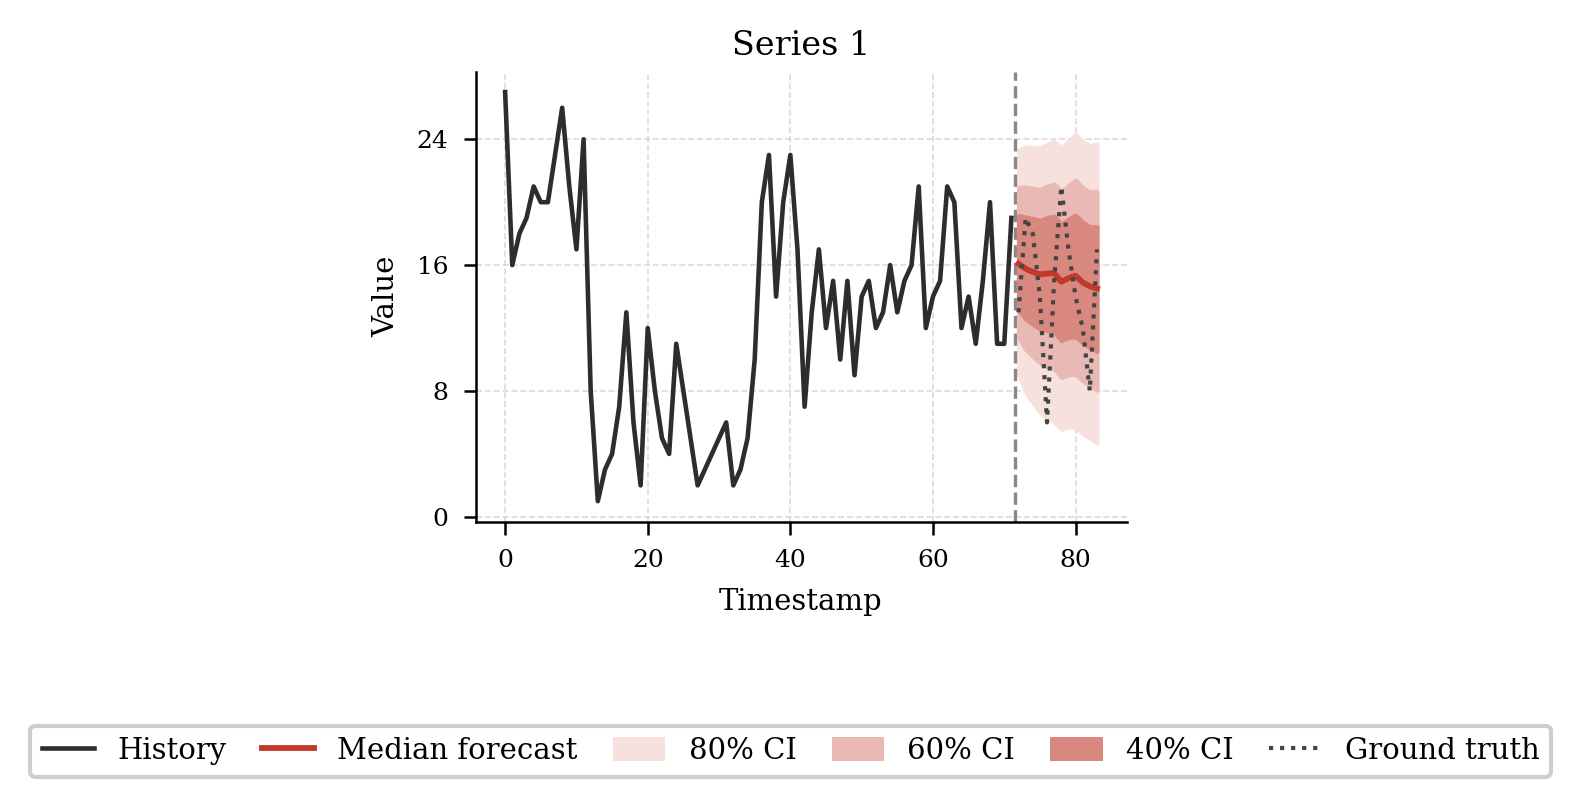
\includegraphics[width=0.8\textwidth]{pictures/hospital.png}
    \caption{Prediction by TabPFN-TS for the hospital dataset. As shown, the time series is very noisy and non-periodic; therefore, the forecast can only capture the trend.}
    \label{fig:hospital_tabpfn_ts_pred}
\end{figure}
In this section, we will further investigate the potential benefits of finetuning TabPFN-TS on the time-series datasets GIFT-Eval and autogluon/chronos-datasets.
For this endeavor, we will examine two methods of finetuning.
The first is finetuning on one dataset.
This will presumably enhance performance on the specific dataset we will train on and potentially other datasets that share some characteristics. %todo
The second method is finetuning on multiple datasets.
As \citet{Hollmann_2025} already showed, finetuning TabPFN across multiple datasets is equivalent to continuing pretraining, thereby enhancing performance across a wide range of datasets.
We will further investigate this by applying the method to time-series data.

\section{Experimental Setup}
%Zuerst daten vorbereitung(dataset_utils)
%daten pro training dataloader
%validation
%hyperparameter setup
%evaluation
For our experiments, we will use full supervised finetuning in which we update all parameters of the model.
This method has been proven to be the best way of finetuning TabPFN since the model is tolerant to full updates and has an insignificant amount of parameters \citep{tanna2026exploring}.

For the most part, the code that is used will be provided by Lennart Purucker's repository ``finetune tabpfn v2''.
Although most of the setup was completed with this, we still had to adjust the normalization of the training error to first make the script work for normal tabular data.
To let the script also finetune on time series data, we also had to make some adjustments in the data creation, batch creation, and validation.

\subsubsection{Data creation/transformation}
GIFT Eval contains 23 datasets, each comprising varying numbers of time series from different domains.
For each dataset, a forecast horizon is defined based on its frequency.
The frequency indicates how often observations are recorded, for example, daily, weekly, or monthly.\newline
Based on this and a predetermined number of sliding windows, training, validation, and test sets can be created for each time series in the dataset.
The test and validation splits have non-overlapping forecast targets to ensure that evaluation and validation are performed on unseen data not included during training.
This means that for a time series with $n$ values, a forecast horizon of $m$ and $w$ windows the training split contains the first $n-(m \cdot (w+1))$ observations, the validation split contains the first $n-(m \cdot w)$ observations and the test split contains all values with the last $(m \cdot w)$ being split into $w$ windows for benchmark evaluation.
This can be seen in the appendix in Figure~\ref{fig:gift_eval_split_us_births_m}.\newline
While only the test data is split into multiple sliding windows, we implemented that the training data is split into $w$ windows as well.
This will be done with the same method as the test split for each time series in a dataset, thus resulting in more training data.
\newline
To finetune TabPFN with time series data in the form of tabular data, we have to transform the data that is selected.
Every time series is transformed into 28 features containing the running index, calendar features, and automatic season features.
This will be done with the code provided by \citet{hoo2025tables} and as it was explained in the background.
\newline
Datasets with time series that do not have a constant length are not taken into account since they require padding to be useful for uniform batch creation.
Since TabPFN-TS was evaluated on GIFT-Eval using a maximum of 4096 points as context length, and for computational purposes, we also clipped all time series to this length.

GIFT-Eval supports three different prediction lengths for almost every dataset, e.g., \ short, medium, and long.
This is done by multiplying the original forecast horizon by different factors that are also based on the frequency of the dataset.
Note that we will only finetune using the short (so the original) forecast horizon, as extending it would exceed the available computational resources.

\subsubsection{Data loading/data selection/batch creation}

As explained in the Background part(here ref), instead of $(x, y)$, one sample consists of a set of n tuples with the form $(x_i, y_i)$.
So in training, one batch consists of $k$ samples, with $k$ also known as the batch size.

The selection of training and validation data fundamentally differs from that of tabular data.
For tabular data, before fine-tuning, one typically randomly selects nnn samples from the dataset and removes them to form the validation set.
Training samples are drawn in a similar way, but remain part of the original dataset.

For time series, the procedure is different.
Each dataset consists of multiple time series, and, as stated earlier, each time series is divided into training, validation, and test splits.

To create a validation set of $k$ predictions, $k$ time series are randomly selected, and their validation splits are used.
After that, we validate every $n$ steps and take the mean of all validation losses of each validation time series.
This validation loss is also used for early stopping, which we configured with a minimum patience of 100 and a maximum patience of 200.

To construct a training batch, one window is randomly sampled from a randomly chosen time series in the current dataset.
This process is repeated kkk times to create a batch of kkk training samples for one epoch.
The same sampling procedure is repeated in every epoch.

\subsubsection{Hyperparameters}
Additionally, to the standard hyperparameters such as batch size and learning rate, we also use a regularizer for the distance to the L2-Starting Point (L2-SP) \citep{xuhong2018explicit}.
Instead of a normal L2 distance, we penalize large deviations from the initial pretrained weights of the model $w^0$.
It is calculated via
\[
    \Omega(w)= \frac{\alpha}{2} \lVert w - w^0 \rVert
\]
where $\alpha$ is the regularization parameter setting the strength of the penalty, thus representing a hyperparameter.
\citet{Hollmann_2025} used it for their continued pretraining, and we wanted to see whether it also improves performance in our experiments

Instead of doing a hyperparameter search first to determine which hyperparameters perform best, we finetune TabPFN 54 times on one dataset for each different hyperparameter configuration.
We use batch sizes 2, 4, 8, 16, 32, and 64 as well as learning rates 0.0005, 0.00005, and 0.000005.
As $\alpha$ for the L2-SP Norm, we use 0, 0.003, and 0.0002.

After that, we take the 5 finetuning checkpoints with the best validation loss and evaluate on the GIFT-Eval evaluation.

\subsubsection{Evaluation}
For evaluation, we use the script provided by TabPFN-TS and only evaluate on short forecast horizons.
Note that we were not able to reproduce all benchmark results that are currently submitted in GIFT-Eval, so before finetuning, we evaluate every dataset on the base checkpoint and take it as a reference.
For the base checkpoint, we use the \textit{tabpfn-v2-regressor-2noar4o2} checkpoint, which was also used in \citet{hoo2025tables}.
To compare the evaluation results, we observe the Mean Absolute Scaled Error(MASE) and take the percentage difference compared to the original checkpoint, and average it for the five finetuning checkpoints.
If this value is negative, we conclude an improvement.
If it is positive, we conclude a worsening.
\section{Results}
This section will present the results of our finetuning experiments while not interpreting them. %TODO
\subsection{Finetuning on one Dataset}
\label{subsec:singlefinetuning}
For finetuning on one dataset, we, as the name suggests, only used data from one dataset.
Since many datasets from GIFT-Eval come with different observation frequencies, we use only the data from one frequency from one dataset, as it was divided in GIFT-Eval.
With this method, we were able to train TabPFN on 33 different datasets with different metadata like context length, time series amount, or forecast horizon.
After completing this procedure, we now have 54 checkpoints for each of the 33 datasets.
This is due to our method of evaluating 54 different configurations for hyperparameter tuning.

%TODO
We report the training summary in Figure~\ref{}, showing that validation loss has improved on all but two datasets.
By looking at each training summary, we can  see that on all except for two datasets, the validation loss improved in at least one of the checkpoints for each dataset.
The two datasets that did not improve regarding the validation loss are jena\_weather with frequency 10T and ett1 with frequency D, both of which are multivariate datasets with 20 and 7 varieties.

%To evaluate whether the fine-tuning process improved or degraded the performance of TabPFN-TS on our dataset, we rank all 54 checkpoints for each dataset according to their validation loss and select the top five.
%This will result in five lists of different error metrics for each dataset, from which we will select the MASE as we mentioned earlier, and the percentage difference to its original checkpoint.
We further evaluated the Top-5 configurations according to validation loss and compare the percentage difference in MASE to the original checkpoint.


As you can see in Figure~\ref{tab:eval_score_single_finetune} is that only 14 finetuning runs led to an improved average performance for every dataset.

Another thing that can be seen in Figure~\ref{tab:eval_score_single_finetune} in the appendix, the order of the checkpoints that were selected via the validation loss is not the same as the order in which they are in evaluation performance.
Not only that, but it also does not always indicate an improvement on the benchmark regarding the dataset if the validation loss itself improved.

An example can be seen in Figure~\ref{fig:eval_M_DENSE_H} by looking at the five evaluated checkpoints of the dataset M\_DENSE with hourly frequency.
\begin{figure}[H]
    \centering
    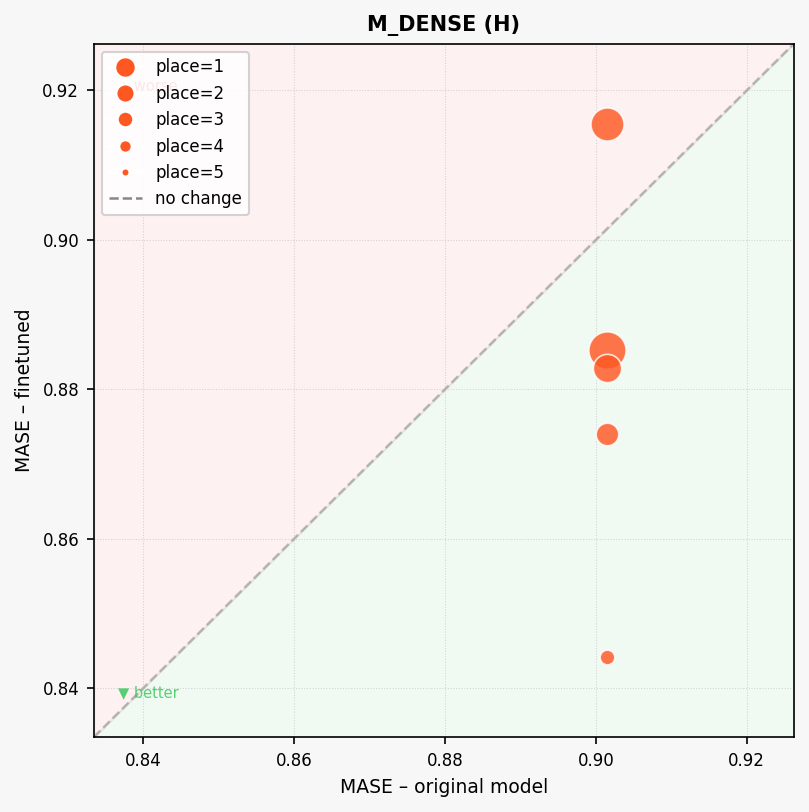
\includegraphics[scale=0.5]{pictures/eval_M_DENSE_H.png}
    \caption{Evaluation results of finetuning with M\_DENSE dataset with hourly frequency. The picture shows an improvement and worsening of the top five checkpoints. As already mentioned, they are not in order regarding the validation loss.}
    \label{fig:eval_M_DENSE_H}
\end{figure}
% TODO prozentual Plot der Verbesserung zeigen Balkendiagramm


\begin{figure}[H]
    \centering

    \begin{subfigure}[t]{0.48\textwidth}
        \centering
        
\includegraphics[width=\linewidth]{pictures/plot1_score_series.pdf}
        \caption{Score Series}
        \label{fig:plot1_score_series}
    \end{subfigure}
    \hfill
    \begin{subfigure}[t]{0.48\textwidth}
        \centering
        
\includegraphics[width=\linewidth]{pictures/plot2_context_vs_series.pdf}
        \caption{Context vs Series}
        \label{fig:plot2_context_vs_series}
    \end{subfigure}

    \caption{Listing of both plots regarding the context length and time series amount. Green marks an improvement, while red indicates performance degradation. }
    \label{fig:combined_plots}
\end{figure}
In Figure~\ref{fig:plot1_score_series} shows the relationship between the total number of observations per dataset and the MASE difference.
For datasets with more than 100,000 observations, the MASE difference is predominantly negative.

Figure~\ref{fig:plot2_context_vs_series} illustrates that datasets with both high context length and many time series are predominantly associated with negative MASE differences.
%If there is a notable amount of time series and a notable amount of context finetuning was successful and improved performance.
Datasets with only one of these characteristics are more frequently associated with positive MASE differences.
This can be observed particularly in datasets containing only a single time series, which, with few exceptions, perform worse than before fine-tuning.

\subsection{Finetuning on multiple Datasets}
\label{subsec:multifinetuning}
Next, we fine-tune TabPFN on multiple time series datasets simultaneously.
This is done by first selecting a handful of datasets we want to use for training, and then for every epoch randomly selecting one dataset we want to build the batch from.
For the next epoch, data from another dataset will be drawn.

Validation is done by validating on every dataset we also use for training, normalizing the error, and adding it together to get a combined validation error for a large number of datasets.

Instead of finetuning TabPFN on a large amount and variety of datasets, we decided to split the datasets into three categories with respect to different context lengths, motivated by \citet{Hollmann_2025}.
They concluded that longer context resulted in better results, and we wanted to validate these results.
We defined the threshold for each category as follows: Small $\rightarrow$ 0-250, Medium $\rightarrow$ 250-1000, Large $\rightarrow$ 1000-Inf.
Note that all time series with a context length greater than 4096 were truncated, as 4096 is the largest context length considered during training, following \citet{hoo2025tables}.

We evaluate our finetuned models in three settings:
The unseen test sets of the datasets it was trained on, unseen datasets from the same category, and unseen datasets from different categories.
%For independent evaluation, we are limited to datasets we did not finetune with.
%This limits most of the categories to only a few datasets.
%So for our plan, we also evaluate on datasets we trained with and datasets from other categories to check if performance improves across the board.
%Both of these are marked in the plots.
\subsubsection{Small Context Length}
For datasets that have a small context length (0-250 observations per time series), we selected the following for training:
\begin{table}[H]
\centering
\begin{tabular}{lrr}
\hline
Dataset & Context Length & Num Series \\
\hline
ett1/W & 103 & 1 \\
hospital & 84 & 767 \\
electricity/W & 208 & 370 \\
covid\_deaths & 212 & 266 \\
ett2/W & 103 & 1 \\
\hline
\end{tabular}
\caption{}
\label{tab:datasets}
\end{table}
Since there are few datasets with a short context length, we were only able to independently evaluate the checkpoints on one dataset.
\begin{table}[H]
\centering
\begin{tabular}{lrr}
\hline
Dataset & Context Length & Num Series \\
\hline
solar/W & 52 & 137 \\
\hline
\end{tabular}
\caption{}
\label{tab:solar_w}
\end{table}
Additionally to this, and as stated above, we will also evaluate on the datasets we trained on, as well as two datasets that are from the medium and big categories.
These two datasets are the following:
\begin{table}[H]
\centering
\begin{tabular}{lrrr}
\hline
Dataset & Context Length & Num Series & Category \\
\hline
LOOP\_SEATTLE/D & 365 & 323 & Medium \\
M\_DENSE/H & 17520 & 30 & Large \\
\hline
\end{tabular}
\caption{}
\label{tab:selected_datasets}
\end{table}
% first run
% list dataset we finetuned with
% list dataset we evaluated with and results
% list datasets we also trained with
\begin{figure}[H]
    \centering
    
\includegraphics[scale=0.7]{pictures/multi_short/mase_mean_delta_plot.png}
    \caption{Horizontal diverging bar chart for multi-dataset fine-tuning with short context length. Lower is better.}
    \label{fig:multi_short_mase_mean_delta_plot}
\end{figure}
\begin{table}[H]
\centering
\resizebox{\textwidth}{!}{
\begin{tabular}{l l c r r r r r r r r r c}
\hline
dataset & context & trained & num & ckpt1 & ckpt2 & ckpt3 & ckpt4 & ckpt5 & mean & min & max & imp \\
\hline
m\_dense/H      & big    & F & 1 & 18.25 & 36.51 & 15.43 & 2.53 & 7.19 & 15.98 & 2.53 & 36.51 & F \\
loop\_seattle/D & medium & F & 1 & 5.87 & 10.17 & 4.17 & \textbf{-1.35} & 2.55 & 4.28 & -1.35 & 10.17 & F \\
solar/W        & short  & F & 1 & \textbf{-1.27} & -0.07 & 2.93 & 3.76 & 44.53 & 9.98 & -1.27 & 44.53 & F \\
hospital/M     & short  & T & 1 & 7.12 & 0.92 & 5.24 & \textbf{-0.46} & 0.56 & 2.68 & -0.46 & 7.12 & F \\
electricity/W  & short  & T & 1 & 4.44 & 8.86 & 6.01 & \textbf{-2.60} & 4.09 & 4.16 & -2.60 & 8.86 & F \\
ett1/W       & short  & T & 7 & -11.15 & -1.99 & \textbf{-13.80} & -9.13 & -11.30 & -9.47 & -13.80 & -1.99 & T \\
covid\_deaths/D & short  & T & 1 & 23.00 & 68.43 & 5.89 & 16.77 & 19.65 & 26.75 & 5.89 & 68.43 & F \\
ett2/W         & short  & T & 7 & 97.35 & 81.49 & 45.00 & 44.82 & 97.17 & 73.16 & 44.82 & 97.35 & F \\
\hline
\end{tabular}
}
\caption{Results of the five checkpoints for multi-dataset fine-tuning with short context length and their percentage difference to the original checkpoint. If a checkpoint resulted in an improvement (negative value), it is shown in bold when it also corresponds to the smallest value.}
\label{tab:multi_short_wide_results}
\end{table}
We report results in Figure~\ref{fig:multi_short_mase_mean_delta_plot} and Table~\ref{tab:multi_short_wide_results}.
As the graph depicts, the mean performance of all 5 best checkpoints performed significantly worse than the original checkpoint on almost all datasets.
The MASE not only worsened on the designated evaluation dataset but also worsened on the dataset we trained with, as well as the two datasets that came from a different category.
The only exception is ett1/W, where we can see a small average improvement of 1,99 percent.
This behavior can be observed across all top 5 checkpoints.
So, all five checkpoints performed almost the same.

\subsubsection{Medium Context Length}
For medium-sized datasets, there was more data available, thus more data to independently evaluate TabPFN on.
But first, for training, we chose the following datasets with their context length and time series amount.
\begin{table}[H]
\centering
\begin{tabular}{lrr}
\hline
Dataset & Context Length & Time Series Length \\
\hline
ett2/D & 725 & 1 \\
sz\_taxi/H & 744 & 156 \\
us\_births/M & 240 & 1 \\
solar/D & 365 & 137 \\
ett1/D & 725 & 1 \\
m\_dense/D & 730 & 30 \\
\hline
\end{tabular}
\caption{}
\label{tab:ctx_ts}
\end{table}
As mentioned before, independent evaluation datasets (so datasets we did not train with) are not as scarce as they were in the short context length category, so we had more datasets to evaluate on.
For evaluation, we chose the following:
\begin{table}[H]
\centering
\begin{tabular}{lrr}
\hline
Dataset & Context Length & Time Series Length \\
\hline
bitbrains\_rnd/H/short & 720 & 500 \\
loop\_seattle/D & 365 & 323 \\
saugeenday/M & 780 & 1 \\
hierarchical\_sales/W & 260 & 118 \\
\hline
\end{tabular}
\caption{}
\label{tab:ctx_ts_2}
\end{table}
And to check whether performance also improved on datasets that were not even in the category, we chose the following two:
\begin{table}[H]
\centering
\begin{tabular}{lrrr}
\hline
Dataset & Context Length & Time Series Length & Category \\
\hline
sz\_taxi/15T & 2976 & 156 & Large\\
covid\_deaths/D & 212 & 266 & Small\\
\hline
\end{tabular}
\caption{}
\label{tab:ctx_ts_3}
\end{table}

%TODO Plots: Mean plot
%TODO table of evaluation
%TODO table of hp
After training, we got the following results over all evaluated datasets
\begin{figure}[H]
    \centering
    
\includegraphics[scale=0.7]{pictures/multi_medium/mase_mean_delta_plot.png}
    \caption{Horizontal diverging bar chart of multi-dataset fine-tuning with short context length. Lower is better.}
    \label{fig:multi_medium_mase_mean_delta_plot}
\end{figure}
The results are completely different from those of short context finetuning.
What is immediately apparent is that, on average across all five checkpoints, 8 out of 12 datasets show a performance improvement.
On all datasets, which we only used for evaluation, TabPFN performed better than the original checkpoint.
Contrary to that, 3 out of 6 datasets we trained TabPFN with experienced a performance loss in the evaluation.

\begin{table}[H]
\centering
\resizebox{\textwidth}{!}{
\begin{tabular}{l l c r r r r r r r r r c}
\hline
dataset & context & trained & num & ckpt1 & ckpt2 & ckpt3 & ckpt4 & ckpt5 & mean & min & max & imp \\
\hline
covid\_deaths/D        & short  & F & 1 & 7.91 & 9.15 & 14.74 & 18.53 & 27.55 & 15.58 & 7.91 & 27.55 & F \\
sz\_taxi/15T           & big    & F & 1 & \textbf{-0.83} & -0.71 & -0.53 & 0.69 & 0.31 & -0.22 & -0.83 & 0.69 & T \\
bitbrains\_rnd/H       & medium & F & 2 & -0.93 & -0.92 & -1.73 & \textbf{-3.00} & -1.91 & -1.70 & -3.00 & -0.92 & T \\
loop\_seattle/D        & medium & F & 1 & \textbf{-2.83} & -2.52 & -1.91 & -0.38 & -0.08 & -1.54 & -2.83 & -0.08 & T \\
saugeen/M             & medium & F & 1 & 0.60 & -0.50 & 1.58 & -0.43 & \textbf{-3.49} & -0.45 & -3.49 & 1.58 & T \\
hierarchical\_sales/W  & medium & F & 1 & \textbf{-1.16} & -0.92 & -0.55 & 1.02 & 0.13 & -0.30 & -1.16 & 1.02 & T \\
ett2/D                & medium & T & 7 & -34.85 & \textbf{-35.17} & -34.10 & -22.96 & -29.19 & -31.26 & -35.17 & -22.96 & T \\
sz\_taxi/H             & medium & T & 1 & -1.89 & \textbf{-1.90} & -1.57 & -0.18 & 0.36 & -1.04 & -1.90 & 0.36 & T \\
us\_births/M           & medium & T & 1 & -5.32 & \textbf{-14.80} & -7.64 & 0.94 & 24.62 & -0.44 & -14.80 & 24.62 & T \\
solar/D               & medium & T & 1 & 1.01 & 1.02 & \textbf{-2.72} & 0.57 & 0.46 & 0.07 & -2.72 & 1.02 & F \\
ett1/D                & medium & T & 7 & 1.27 & 0.17 & 6.21 & 1.18 & 2.23 & 2.21 & 0.17 & 6.21 & F \\
m\_dense/D             & medium & T & 1 & \textbf{-0.52} & 0.00 & 1.65 & 4.04 & 5.94 & 2.22 & -0.52 & 5.94 & F \\
\hline
\end{tabular}
}
\caption{Results of the five checkpoints for multi-dataset fine-tuning with medium context length. If a checkpoint resulted in an improvement (negative value), it is shown in bold when it also corresponds to the smallest value.}
\label{tab:medium_context_wide_results}
\end{table}
By looking at~\ref{tab:medium_context_wide_results}, we can see that checkpoint 2 performs best out of the 5 checkpoints we evaluated on.
Checkpoints 4 and 5 performed on average worse and only improved performance on 6 and 7 datasets.
The dataset of the short category performed worse on all checkpoints.

\begin{table}[H]
\centering
\resizebox{\textwidth}{!}{
\begin{tabular}{l r r r r r r r r r r r l r r}
\hline
ckpt & Time & LR & BS & L2-SP & WD & TimeTot & InitLoss & BestLoss & LastLoss & Steps & BestStep & ES Reason & t/step & Util \\
\hline
ckpt\_1 & 2400 & 5e-05 & 32 & 0.0 & 0.0 & 531.13 & 0.3873 & 0.3327 & 0.3361 & 470 & 259 & AdaptiveES & 1.13 & 98.78 \\
ckpt\_2 & 2400 & 5e-05 & 32 & 0.0001 & 0.0 & 513.75 & 0.3873 & 0.3330 & 0.3409 & 450 & 249 & AdaptiveES & 1.14 & 98.84 \\
ckpt\_3 & 2400 & 5e-05 & 8 & 0.0001 & 0.0 & 267.59 & 0.3873 & 0.3352 & 0.3511 & 520 & 309 & AdaptiveES & 0.51 & 88.65 \\
ckpt\_4 & 2400 & 0.0005 & 32 & 0.0001 & 0.0 & 564.65 & 0.3873 & 0.3358 & 0.3632 & 500 & 299 & AdaptiveES & 1.13 & 98.67 \\
ckpt\_5 & 2400 & 0.0005 & 16 & 0.0015 & 0.0 & 343.30 & 0.3873 & 0.3360 & 0.3412 & 490 & 289 & AdaptiveES & 0.70 & 96.84 \\
\hline
\end{tabular}
}
\caption{Training Runs mit verschiedenen Checkpoints}
\label{tab:medium_context_training_ckpts}
\end{table}

The hyperparameters are also an interesting topic to look at.
\ref{tab:medium_context_training_ckpts} showed that 4 out of 5 checkpoints used the L2-SP lambda also used in \ref{realtabpfn}.
Checkpoints 4 and 5 used a learning rate of 0.0005, contrary to checkpoints 1-3, which used 0.00005.

% im mean wird es auf 8 besser und auf 4 schlechter
% auf 3 datensets auf denen auch trainiert wurde wurde es schlechter
% auf datensets auf denen nicht trainiert wurde und nur evaluiert wurde und auch medium length haben wurde es nur besser bzw ziemlich gleich
%
% checkpoint 2 performed am besten über alle datensets
% checkpoints 4 und 5 performen schlechter als der durchschnitt
% auf short viel verschlechtert und auf big context length nicht signifikant verbessert aber auch nicht verschlechtert
% bei hyperparametern sind l2 sp lambda in 4/5 checkpoints drin
% da ckpt 4 und 5 schlechter performen und lr 0.0005 haben schlechter im vergleich zu 0.00005
% TODO prozentual plot der verbesserung zeigen balken diagramm
%
\subsubsection{Big Context Length}
% list dataset we finetuned with
% list the dataset we evaluated with
% list datasets we also trained with
The last multi-finetuning category is of the big context length category.
All datasets in this category consist of time series with a context length of at least 1000 observations.
So, for training, we chose the following ones.
\begin{table}[H]
\centering
\begin{tabular}{lrr}
\hline
Dataset & Context Length & Time Series Length \\
\hline
hierarchical\_sales/D & 1825 & 118 \\
electricity/D & 1461 & 370 \\
sz\_taxi/15T & 2976 & 156 \\
m\_dense/H & 17520 & 30 \\
\hline
\end{tabular}
\caption{}
\label{tab:ctx_ts_4}
\end{table}
As well as the medium category, the large context length category also provides more datasets than the short context length category, so we will have more datasets to independently evaluate on.
For evaluation, we take:
\begin{table}[H]
\centering
\begin{tabular}{lrr}
\hline
Dataset & Context Length & Time Series Length \\
\hline
saugeenday/D/short & 23741 & 1 \\
us\_births/D/short & 7305 & 1 \\
ett1/15T & 69680 & 1 \\
ett1/H & 17420 & 1 \\
ett2/H & 17420 & 1 \\
ett2/15T & 69680 & 1 \\
\hline
\end{tabular}
\caption{}
\label{tab:ctx_ts_5}
\end{table}
To evaluate whether the trained checkpoints also improved on datasets that are not in the same category (so they have fewer observations than 1000), we also evaluate on these two datasets.
\begin{table}[H]
\centering
\begin{tabular}{lrrr}
\hline
Dataset & Context Length & Time Series Length & Category \\
\hline
covid\_deaths/D & 212 & 266 & Small\\
loop\_seattle/D & 365 & 323 & Medium\\
\hline
\end{tabular}
\caption{}
\label{tab:ctx_ts_6}
\end{table}
%TODO Plots: Mean plot
%TODO table of evaluation
%TODO table of hp
Our evaluation emitted the following results:
\begin{figure}[H]
    \centering
    
\includegraphics[scale=0.7]{pictures/multi_big/mase_mean_delta_plot.png}
    \caption{Horizontal diverging bar chart of multi-dataset fine-tuning with short context length. Lower is better.}
    \label{fig:multi_medium_mase_mean_delta_plot}
\end{figure}
8 out of 12 datasets show improved average results over all checkpoints compared to the original checkpoint.
But on most of these datasets, the improvement is not as significant as that of others.
Looking at the evaluation datasets, we see that 4 out of 6 datasets show an improvement compared to the original.

The short dataset also became worse than the original.

\begin{table}[H]
\centering
\resizebox{\textwidth}{!}{
\begin{tabular}{l l c r r r r r r r r r c}
\hline
dataset & context & trained & num & ckpt1 & ckpt2 & ckpt3 & ckpt4 & ckpt5 & mean & min & max & imp \\
\hline
covid\_deaths/D       & short & F & 1 & 23.56 & 77.34 & 49.68 & 49.19 & 44.23 & 48.80 & 23.56 & 77.34 & F \\
loop\_seattle/D       & medium& F & 1 & -1.92 & -1.96 & \textbf{-2.80} & -2.62 & -2.07 & -2.27 & -2.80 & -1.92 & T \\
ett1/15T             & big   & F & 7 & -2.98 & -5.00 & \textbf{-7.94} & -7.19 & -5.88 & -5.80 & -7.94 & -2.98 & T \\
ett1/H               & big   & F & 7 & -0.03 & \textbf{-4.94} & -2.68 & -2.64 & -2.60 & -2.58 & -4.94 & -0.03 & T \\
saugeen/D            & big   & F & 1 & 1.82 & -2.55 & \textbf{-4.33} & -2.01 & 2.08 & -1.00 & -4.33 & 2.08 & T \\
ett2/H               & big   & F & 7 & -1.79 & \textbf{-4.05} & -0.47 & -0.81 & 2.61 & -0.90 & -4.05 & 2.61 & T \\
ett2/15T             & big   & F & 7 & 1.77 & -0.42 & \textbf{-1.67} & -1.36 & 0.20 & -0.30 & -1.67 & 1.77 & T \\
us\_births/D          & big   & F & 1 & 34.64 & 20.01 & -- & 20.01 & 19.44 & 23.53 & 19.44 & 34.64 & F \\
hierarchical\_sales/D & big   & T & 1 & -1.35 & -1.44 & -0.33 & -0.30 & \textbf{-1.62} & -1.01 & -1.62 & -0.30 & T \\
electricity/D        & big   & T & 1 & 1.65 & \textbf{-3.18} & -0.77 & -0.63 & -0.45 & -0.68 & -3.18 & 1.65 & T \\
sz\_taxi/15T          & big   & T & 1 & 0.05 & \textbf{-0.27} & 0.20 & 0.22 & 0.05 & 0.05 & -0.27 & 0.22 & F \\
m\_dense/H            & big   & T & 1 & 1.01 & -1.63 & 2.12 & 2.10 & \textbf{-2.21} & 0.28 & -2.21 & 2.12 & F \\
\hline
\end{tabular}
}
\caption{Results of the five checkpoints for multi-dataset fine-tuning with large context length. If a checkpoint resulted in an improvement (negative value), it is shown in bold when it also corresponds to the smallest value.}
\label{tab:wide_results_3}
\end{table}
By looking at~\ref{tab:wide_results_3}, we can see that checkpoint 2 performed best out of all datasets and checkpoint 1 performed worst.
% 4/6 individuellen Datensets wurde es besser bzw. hat sich nicht verschlechtert
% 7 Datensets wurden besser. Davon 2, auf denen auch trainiert wurde.


% TODO prozentual Plot der Verbesserung zeigen Balkendiagramm

\section{Discussion}
The first research question we developed in the expose is ``Can we finetune TabPFN for time series with time-series data (and does it improve the performance)?''.
Our results that we got by finetuning TabPFN-TS on all 33 datasets of GIFT-Eval indicate that this question can be answered with a yes.
But it is dependent on the structure and features of the dataset.

% Validation Loss nicht richtige Order bzw. Indikator, dass Validierung besser ist
We first examine the significance of the validation loss for improved evaluation results.
As mentioned in the results section, we saw few to no correlations between the order of checkpoints regarding the validation loss and the order of them regarding the evaluation loss.
For example, in Figure~\ref{fig:eval_M_DENSE_H} we saw that the fifth checkpoint outperforms all of the other four checkpoints that were selected in order of validation loss.
Firstly, this is likely because the validation loss is MSE, whereas for evaluation we use the MASE.
Secondly, it is also because the data most likely overfits the validation data.
Datasets with one time series often halve their validation loss but show worsening in evaluation (e.g., see results on datasets). %TODO

By looking at Figure~\ref{fig:plot1_score_series}, we saw that the number of observations in one dataset highly correlates with the improvement we get from finetuning.
If a dataset has more than 100 thousand total observations, finetuning will most likely succeed by improving the evaluation loss.
%Hier nochmal theoretischen Teil mit Paper
Results in Figure~\ref{fig:plot2_context_vs_series}, further confirm this trend showing that finetuning on large context sizes and large amount of time series often improve performance.%where one can see a correlation between a large amount of context per series and a large amount of time series in a dataset, and an improved performance.
This now not only indicates that the number of observations contributes to an improved finetuning run, but also the structure of the dataset itself by providing multiple time series with a certain amount of datapoints.
\newline
Time series datasets differ from standard tabular datasets in that the tables within a dataset stem from the same domain and share a common distribution.
A longer individual time series does not necessarily lead to better fine-tuning (with some exceptions).
However, providing multiple time series (and thus multiple tables) appears to benefit fine-tuning.
An example is weather forecasting: having observations from multiple weather stations within the same city provides more information, as different stations exhibit variation in their measurements while still following nearly the same underlying distribution.

%failure cases
There are some exceptions to this.
We identified two tasks characteristics that make finetuning harder: Noisy datasets and intermittent data.
If we take a look at the hospital dataset that we also used as an example in Figure~\ref{fig:hospital_tabpfn_ts_pred}, we can see a small downwards trend but not periodicities.
This characteristic is typical for a noisy dataset: Random fluctuations that make it difficult for any forecasting model to predict.
This has been observed in prior work reporting that time series forecasting models have problems predicting on noisy datasets, as they were mostly trained on well-composed time series and have a hard time finding a schema in these data \citep{gupta2025evaluating}.
\newline
% TODO Soll ich überhaupt drinlassen?
Other datasets show other characteristics that make it hard for TabPFN to train on.
Looking at~\ref{bizitop_TODO}, we can see that in this dataset, a signal emerges periodically, but not in the same amplitude every time.
Between those signals, the values of the time series are constantly at or near zero.
This type of data is called intermittent data.
\citet{KieferGrimmBaueretal_2021} talked about this issue and came to the conclusion that deep learning approaches perform well, but still struggle to fully adapt to this type of data.
This could be a cause for TabPFN to not be able to finetune well on this type of data, as it was not able to find a good structure in this data.
%- schlecht zu quantifizieren aber Datensätze mit Time Series die sehr "noisy"(also nicht vorausschaubar) sind funktionieren nicht so gut weil TabPFN kein Schema finden kann (hier vielleicht https://arxiv.org/abs/2501.00889 aber das Paper sieht bisschen komisch aus)
%- Wenn Signal nur sehr selten kommt und dazwischen das Signal "konstant" ist, lernt es auch schlecht (intermittent Daten) https://link.springer.com/article/10.1007/s10479-023-05447-7
%hier erklären
% especially datasets with challenging structure were bad at finetuning
Overall, these results show that finetuning TabPFN-TS on real-world time series data can improve forecasting performance, but only under certain conditions.
In particular, success depends strongly on dataset size, structure, and signal quality, while noisy or intermittent datasets remain challenging.

\iffalse
- immer mit Research-Frage anfangen
- Fine-tuning on one dataset teuer weil viele Hyperparameter und nicht die eine Hyperparameter Config gefunden wurde
- dass der Validation Loss bei allen runtergeht aber die Evaluation nicht immer klappt lässt sich mit Overfitting auf den Validation Sets erklären
- Das sieht man vor allen Dingen bei den Datensets, die nur eine Zeitreihe haben -> Validation Loss wird manchmal halbiert, aber Evaluation viel schlechter
- Wenn das Signal nur sehr selten kommt und dazwischen das Signal "konstant" ist, lernt es auch schlecht (intermittent Daten) https://link.springer.com/article/10.1007/s10479-023-05447-7
- conclusion -> Es geht aber es gibt limitations durch Charakteristiken von Datensets und ihren Time Series
\fi

The question we investigate in our multi-dataset fine-tuning experiments is:
"Can we further improve performance by finetuning on multiple datasets similar to RealTabPFN \citep{Hollmann_2025}?"
This question can be answered with a yes, although not every category we established equally helped train the model to perform better on our evaluation datasets.
In the upcoming section, we will assess the different categories and finally compare them to single finetuning.

Finetuning with the small context lengths category only led to worsening.
This can be observed not only in our evaluation datasets but also in almost all datasets we trained on, including those from the multi and big categories.
This result goes hand in hand with the results also obtained by \citep{Hollmann_2025}.
A possible reason for this is the lack of information we have due to the smaller context.
TabPFN is not able to identify underlying structures in the data, thus generating a noisier gradient.
\newline
Another possibility is the differences regarding the characteristics of the time series.
Given that the context length is already small, it is also problematic that this occurs.

In contrast, the medium category achieved the best results out of all three methods.
Based on the five checkpoints, TabPFN-TS improved on average on nearly all evaluation datasets.
This is likely due to a larger number of datasets in this category, as well as more equally distributed characteristics that make it easier for TabPFN to learn with.
\newline
This performance does not distribute equally across all five checkpoints; it applies only to the first two.
An important factor that separates these two checkpoints from the other lower-performing ones is the learning rate.
The first two trained with a learning rate of 0.00005, while the other three trained with a learning rate of 0.0005.
This suggests that a more conservative approach with lighter updates suits TabPFN finetuning better in this context length setting.
% TODO average context length

For the training run we did with datasets from the large context-length category, we also achieved significant improvements in performance.
Although they were more subtle than the ones we had with the medium context length.
It can also be observed that the small-context-length dataset evaluation resulted in performance degradation, whereas the evaluation run with the medium context-length dataset showed improved performance.
This reinforces our theory that, for small-context-length datasets, TabPFN does not achieve satisfying performance boosts after finetuning across multiple datasets with any context length.
\newline
\citet{Hollmann_2025} observed an increase in downstream accuracy with larger context sizes when finetuning TabPFN across multiple tabular datasets.
Despite also seeing a large increase in accuracy from small to medium context length, we did not see the same leap from medium to large context size.
This could be due to a different technical setup than the one used in their work, or to the fact that we fine-tuned using time-series data and the effects that result from it.
However, this requires further investigation.


% 2. Small context length results
% 3. Medium context length results
% 4. Big context length results
% 5. HP LR 0.00005 besser als 0.0005 und L2 SP lambda -> instabiler, lieber konservativeres Training

% 1. High-level summary
% 5. rolle der Datenheterogenität
% 6. Transfer zwischen Kategorien
% 7. limitations: wenige unabhängige Datensets, starker Datenset-Auswahl-Trainings-Bias

% 8. Conclusion: sinnvoll für Generalisierung, wirkt wie lightweight Pretraining


% Single besser für einzelne dafür Multi besser für Generalisierung

% Nur weil auf Datensets trainiert wird heißt es nicht dass es auch besser wird für Multi

% Multi funktioniert auf Medium Datensets am besten dann Big geht bisschen und Small geht gar nicht
% Aber das kann zum Teil auch an Datensets liegen auf denen es einfach besser funktioniert

% Hyperparameter kann man nicht so gut fassen weil es zwischen allen Läufen anders ist welche gut sind und wie lange sie brauchen
% Wenn Multi-Finetuning funktioniert dann hilft es auch zum Teil für Datensets die gar nicht im Fokus für das Training waren
% funktionieren also wie eine Art Prior zum Teil und deshalb wird für Time Series Data dass von real tabpfn zum Teil bestätigt
% Small: → „funktioniert gar nicht / Overfitting / kein Transfer“
%However, as can be seen in~\ref{tab:datasets} ett1/W also was a dataset we trained on.

% Medium: → „beste Generalisierung“
%lr vielleicht 0,00005 besser als 0.0005

% Big: → „stabil aber wenig Gain“

%limitations: „wenig eval Datensets, weil viele für Training genutzt wurden“